 %! TeX program = lualatex

\documentclass[letterpaper]{article}
\usepackage[dvipsnames]{xcolor}
\usepackage{amsmath}
\usepackage{amssymb}
\usepackage{enumitem}
\usepackage[margin=1.5in]{geometry}
\usepackage{graphicx}
% \usepackage{helvet}
% \renewcommand{\familydefault}{\sfdefault}
\usepackage{newtxsf}
\usepackage[most]{tcolorbox}

\usepackage{fontspec}

\usetikzlibrary{decorations.pathmorphing}


\graphicspath{ {../images/} }

%TODO Title
\def\T{Chapter 3: Set Theory}
%TODO Day
\def\D{10}
%TODO Month
\def\M{9}
%TODO Year
\def\Y{2024}
\addtolength{\topmargin}{-4in}
\setlength{\topmargin}{0pt}
\title{\vspace{-3.0cm}\textbf{\T}}
\date{\vspace{-1cm}}
\author{~}



\tcbset{
%%%%%% HALF frame corner styles (produces half a corner) %%%%%%
    % North West frame corner - Left segment only
    frame corner northwest left/.style n args={5}{
        frame code app={
            % \shade[top color={#4},bottom color={#5}]
            %     ([xshift={-#3},yshift={-#1}]frame.north west)
            %     --++(0,{#1+#3})
            %     --++({#2},{-#2})
            %     --++(0,{-#1+#2-#3})
            %     --cycle;
            % \node at ([xshift={-#3},yshift={-#1}]frame.north west) {hi};
            \draw [rounded corners, line width=2mm]
                ([xshift={-#3},yshift={-#1}]frame.north west) --
                ([xshift={-#3},yshift={#3}]frame.north west) --
                ([xshift={#1},yshift={#3}]frame.north west);
        }
    },
    % North West frame corner - Top segment only
    frame corner northwest top/.style n args={5}{
        frame code app={
            \shade[left color={#4},right color={#5}]
                ([xshift={#1},yshift={#3}]frame.north west)
                --++({-#1-#3},0)
                --++({#2},{-#2})
                --++({#1-#2+#3},0)
                --cycle;
        }
    },
    % North East frame corner - Right segment only
    frame corner northeast right/.style n args={5}{
        frame code app={
            \shade[top color={#4},bottom color={#5}]
                ([xshift={#3},yshift={-#1}]frame.north east)
                --++(0,{#1+#3})
                --++({-#2},{-#2})
                --++(0,{-#1+#2-#3})
                --cycle;
        }
    },
    % North East frame corner - Top segment only
    frame corner northeast top/.style n args={5}{
        frame code app={
            \shade[right color={#4},left color={#5}]
                ([xshift={-#1},yshift={#3}]frame.north east)
                --++({#1+#3},0)
                --++({-#2},{-#2})
                --++({-#1+#2-#3},0)
                --cycle;
        }
    },
    % South West frame corner - Left segment only
    frame corner southwest left/.style n args={5}{
        frame code app={
            \shade[bottom color={#4},top color={#5}]
                ([xshift={-#3},yshift={#1}]frame.south west)
                --++(0,{-#1-#3})
                --++({#2},{#2})
                --++(0,{#1-#2+#3})
                --cycle;
        }
    },
    % South West frame corner - Bottom segment only
    frame corner southwest bottom/.style n args={5}{
        frame code app={
            \shade[left color={#4},right color={#5}]
                ([xshift={#1},yshift={-#3}]frame.south west)
                --++({-#1-#3},0)
                --++({#2},{#2})
                --++({#1-#2+#3},0)
                --cycle;
        }
    },
    % South East frame corner - Right segment only
    frame corner southeast right/.style n args={5}{
        frame code app={
            \shade[bottom color={#4},top color={#5}]
                ([xshift={#3},yshift={#1}]frame.south east)
                --++(0,{-#1-#3})
                --++({-#2},{#2})
                --++(0,{#1-#2+#3})
                --cycle;
        }
    },
    % South East frame corner - Bottom segment only
    frame corner southeast bottom/.style n args={5}{
        frame code app={
            \shade[right color={#4},left color={#5}]
                ([xshift={-#1},yshift={-#3}]frame.south east)
                --++({#1+#3},0)
                --++({-#2},{#2})
                --++({-#1+#2-#3},0)
                --cycle;
        }
    },
}

\tcbset{
    frame corners northwest rounded/.style n args={4}{
        frame code app={
            \draw [rounded corners=2mm, line width=2mm, color={#4}]
                ([xshift={-#3},yshift={-#1}]frame.north west) --
                ([xshift={-#3},yshift={#3}]frame.north west) --
                ([xshift={#1},yshift={#3}]frame.north west);
        }
    },
    % South East frame corner - Both segments (right and bottom)
    frame corners southeast/.style n args={4}{
        frame code app={
            \draw [rounded corners=2mm, line width=2mm, color={#4}]
                ([xshift={#3},yshift={#1}]frame.south east) --
                ([xshift={#3},yshift={-#3}]frame.south east) --
                ([xshift={-#1},yshift={-#3}]frame.south east);
        }
    },
    frame corners lr rounded/.style n args={4}{
        frame corners northwest rounded={#1}{#2}{#3}{#4},
        frame corners southeast={#1}{#2}{#3}{#4},
    }
}

% \newtcolorbox{hdefbox}[3][]{%
%   colback=RoyalBlue!5!white,
%   coltitle=RoyalBlue!15!black,
%   title filled=false,
% 	enhanced,
%   detach title,
%   tile,
%   before upper={\tcbtitle\medskip\\},
%   borderline={2pt}{0pt}{
%     draw=blue!40!black,
%     decorate,
%     decoration={random steps,segment length=2pt,amplitude=0.4pt}
%   },
%   arc=0mm,
% 	title={Definition~#2~#3},
% 	#1
% }

\newtcolorbox{defbox}[3][]{%
  colback=RoyalBlue!5!white,
  coltitle=RoyalBlue!15!black,
  title filled=false,
	enhanced,
  detach title,
  tile,
  before upper={\tcbtitle\medskip\\},
  borderline west={2mm}{0pt}{RoyalBlue},
  % attach boxed title to top center={yshift=-2mm},
  leftrule=2mm,
  toprule=0mm,
  bottomrule=0mm,
  rightrule=0mm,
  arc=0mm,
	title={Definition~#2~#3},
	#1
}

\newtcolorbox{axbox}[3][]{%
  colback=WildStrawberry!5!white,
  coltitle=WildStrawberry!15!black,
  title filled=false,
	enhanced,
  detach title,
  tile,
  before upper={\tcbtitle\medskip\\},
  borderline west={2mm}{0pt}{WildStrawberry},
  % attach boxed title to top center={yshift=-2mm},
  leftrule=2mm,
  toprule=0mm,
  bottomrule=0mm,
  rightrule=0mm,
  arc=0mm,
	title={Axiom~#2~#3},
	#1
}

\newtcolorbox{lebox}[3][]{%
  colback=Goldenrod!5!white,
  coltitle=Goldenrod!15!black,
  title filled=false,
	enhanced,
  detach title,
  tile,
  before upper={\tcbtitle\medskip\\},
  borderline west={2mm}{0pt}{Goldenrod},
  % attach boxed title to top center={yshift=-2mm},
  leftrule=2mm,
  toprule=0mm,
  bottomrule=0mm,
  rightrule=0mm,
  arc=0mm,
	title={Lemma~#2~#3},
	#1
}

\newtcolorbox{prbox}[3][]{%
  colback=Lavender!5!white,
  coltitle=Lavender!15!black,
  title filled=false,
	enhanced,
  detach title,
  tile,
  before upper={\tcbtitle\medskip\\},
  borderline west={2mm}{0pt}{Lavender},
  % attach boxed title to top center={yshift=-2mm},
  leftrule=2mm,
  toprule=0mm,
  bottomrule=0mm,
  rightrule=0mm,
  arc=0mm,
	title={Proposition~#2~#3},
  breakable,
	#1
}








\begin{document}

\setmainfont{NotoSans-Regular}[
  Path           = /home/snouflake/.fonts/ ,
  Extension      = .ttf ,
  BoldFont       = NotoSans-Bold ,
  ItalicFont     = NotoSans-Italic ,
  BoldItalicFont = NotoSans-BoldItalic,
  ] 

\maketitle

\section*{Fundamentals}

\begin{defbox}{3.1.1}{(Sets, "$\in$")}
  A set is any unordered collection of objects. If $x$ is an object and $A$ is a set, $x \in A \lor x \notin A$.
\end{defbox}

\begin{axbox}{3.1}{Sets are objects}
  If $A$ is a set, then $A$ is also an object; $A$ can belong to $B$, i.e. $\{3,\{3,4\},4\}$
\end{axbox}

\begin{axbox}{3.2}{(Equality of Sets)}
  $A = B \iff \forall x \in A x \in B \land \forall y \in B y \in A$
\end{axbox}

\begin{axbox}{A.7}{(Substitution)}
  If $a$ and $b$ are of the same type and $a = b$, then $f(a) = f(b)$ for all functions and operations $f$. The same applies to any property $P$.
\end{axbox}

It is important to note that the axiom of substitution applies to "$\in$". Therefore, it also applies to all operations we define exclusively in terms of it.

\begin{axbox}{3.3}{(Empty Set)}
  There exists a set $\emptyset \text{ (or $\{\}$) } ~s.t.~ \forall x, x \notin \emptyset$.
\end{axbox}

\begin{lebox}{3.1.5}{(Single Choice)}
  Let $A$ be a non-empty set. $\Rightarrow \exists x ~s.t.~ x \in A$.
  \begin{paragraph}{Proof:} 
    (By contradiction)

    Suppose $\nexists x \in A$.
    $\to \forall x, x \notin A$.
    Also by axiom 3.3, $x \notin A$.
    
    \[
      \text{"Thus, } x \in A \iff x \in \emptyset.\text{"}
    \]

    (Every element of $A$ is in $\emptyset$ and vise versa; axiom 3.2.)
    
    Thus, $A = \emptyset$, a contradiction. $\square$
  \end{paragraph}
\end{lebox}

\begin{axbox}{3.4}{(Singleton and Pair Sets)}
  $\forall a ~\exists ~\{a\}; \forall y, y \in \{a\} \iff y = a$.
  We call $\{a\}$ the singleton set whose element is $a$.

  \medskip

  $\forall a,b ~\exists~ \{a,b\}; \forall y, y \in \{a,b\} \iff (y = a \lor y = b)$
\end{axbox}

Because by axiom 3.2, $\{a,a\} = \{a\}$, the singleton set axiom is redundant.

\begin{axbox}{3.5}{(Pairwise Union)}
  Let $A$ and $B$ be sets. $\exists A \cup B ~s.t.~ x \in A \cup B \iff (x \in A \lor x \in B)$.
\end{axbox}

\begin{lebox}{3.1.12}{~}
  $\forall a,b ~  \{a,b\} = \{a\} \cup \{b\}$.

  $A \cup B = B \cup A$.

  $(A \cup B) \cup C = A \cup (B \cup B)$.

  \begin{paragraph}{Proof:}
    I'm not going to write the proofs here, but the main idea seems to be to split the proof into two cases: for $A \cup B$, when $x \in A$ and when $x \in B$.
  \end{paragraph}
\end{lebox}

\begin{defbox}{3.1.14}{(Subsets)}
  Let $A, B$ be sets.

  $A \subseteq B \iff \forall x \in A, x \in B$. ($A$ is a subset of $B$)

  $A \subsetneq B \iff (A \subseteq B \land A \neq B)$. ($A$ is a proper subset of $B$)
\end{defbox}

Because all of the above is defined in terms of $\in$, it follows the axiom of substitution.

\begin{prbox}{3.1.17}{(Sets are partially ordered by set inclusion)}
  \vspace{-0.5cm}
  \begin{enumerate}
    \item $(A \subseteq B \land B \subseteq C) \Rightarrow A \subseteq C$.
    \item $(A \subseteq B \land B \subseteq A) \Rightarrow A = B$.
    \item $(A \subsetneq B \land B \subsetneq C) \Rightarrow A \subsetneq C$.
  \end{enumerate}

  \begin{paragraph}{Proof (1):}
    We \textbf{choose} an arbetrary element of $A$, $x$. Since $A \subseteq B$, $x \in B$, and since $B \subseteq C$, $x \in C$. Thus any element of $A$ is an element of $C$. $\square$
  \end{paragraph}

\vspace{7cm}

  \begin{paragraph}{Proof (3):}
    Since $(X \subsetneq Y)\Rightarrow (X \subseteq Y), A \subseteq B \land B \subseteq C$. Therefore, by Tao's proof of \textbf{1}, $A \subseteq C$.

    \medskip

    Thus, to show $A \subsetneq C$, we only need show $A \neq C$.

    \medskip

  \end{paragraph}

  \begin{center}
    \begin{tcolorbox}[enhanced,
      frame hidden,
      frame corners lr rounded={5mm}{4.3pt}{5pt}{Lavender},
      width=8cm,
      colback=white,
      opacityback=1,
      ]
      If $(X \subseteq Y \land X \neq Y) \Rightarrow$
      \[
        \left[
          \begin{array}{ccc}
            (\forall x \in X, x \in Y) &
            \land &
            \sim (\forall y \in Y, y \in X)
          \end{array}
        \right]
      \]
      \vspace{-0.4cm}
      \bgroup
        \tiny
        \begin{center}
          \textcolor{Lavender!90!black}{
            \begin{tabular*}{0.8\textwidth}{@{\extracolsep{\fill}} c c}
              If this were false, $X \nsubseteq Y$.
            &
            If this were true, $X = Y$.
            \end{tabular*}
          }
        \end{center}
      \egroup
      \bgroup
      \begin{center}
        \footnotesize
        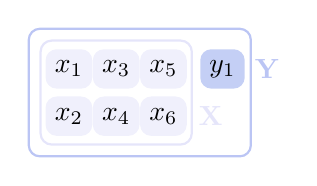
\begin{tikzpicture}[scale=0.6]
          \draw[thick,Lavender,rounded corners] 
          (-0.6,-0.6) -- (2.6,-0.6) -- (2.6,1.6) -- (-0.6,1.6) -- cycle;
          \draw[thick,Lavender!74!RoyalBlue,rounded corners]
          (-0.85,-0.85) -- (3.85,-0.85) -- (3.85,1.85) -- (-0.85,1.85) -- cycle;
          \node at (0,1) [rounded corners,rectangle,minimum width=0.5cm,minimum height=0.5cm,fill=Lavender!60!white]
          {$x_1$};
          \node at (0,0) [rounded corners,rectangle,minimum width=0.5cm,minimum height=0.5cm,fill=Lavender!60!white]
          {$x_2$};
          \node at (1,1) [rounded corners,rectangle,minimum width=0.5cm,minimum height=0.5cm,fill=Lavender!60!white]
          {$x_3$};
          \node at (1,0) [rounded corners,rectangle,minimum width=0.5cm,minimum height=0.5cm,fill=Lavender!60!white]
          {$x_4$};
          \node at (2,1) [rounded corners,rectangle,minimum width=0.5cm,minimum height=0.5cm,fill=Lavender!60!white]
          {$x_5$};
          \node at (2,0) [rounded corners,rectangle,minimum width=0.5cm,minimum height=0.5cm,fill=Lavender!60!white]
          {$x_6$};
          \node at (3.25,1) [rounded corners,rectangle,minimum width=0.5cm,minimum height=0.5cm,fill=Lavender!49!white!74!RoyalBlue]
          {$y_1$};
          \node at (3,0) [color=Lavender]
          {\textbf{X}};
          \node at (4.2,1) [color=Lavender!74!RoyalBlue]
          {\textbf{Y}};
        \end{tikzpicture}
      \end{center}
      \egroup

      $\therefore \exists \text{ some } y \in Y ~s.t.~ y \notin X$.
    \end{tcolorbox}
  \end{center}

  $\therefore (A \subsetneq B) \Rightarrow \exists b \in B ~s.t.~ b \notin A$

  $\therefore (B \subsetneq C) \Rightarrow b \in C \land \exists c \in C ~s.t.~ (c \notin B \land c \notin A \text{ because } A \subseteq B)$

  $\therefore b,c \notin A \land b,c \in C \therefore A \neq C ~\square$

\end{prbox}

\begin{axbox}{3.6}{(Specification)}
  Let $A$ be a set, and $P(x)$ $s.t.$ $\forall x \in A$, $P(x)$ is true or false.

  $\exists~ \{ x \in A : P \text{ (is true)} \}$ s.t.

  \[
    y \in \left\{
      x \in A: P(x)
    \right\}
    \iff
    \left(
      y \in A \land P(y)
    \right)
  \]

\end{axbox}

\begin{defbox}{3.1.22}{(Intersections)}
  \[
    S_1 \cap S_2 := \{ x \in S_1 : x \in S_2 \};
  \]
  \[
    x \in S_1 \cap S_2 \iff x \in S_1 \land x \in S_2.
  \]
\end{defbox}

\begin{defbox}{3.1.26}{(Difference sets)}
  \[
    A - B := \{ x \in A : x \notin B \}
  \]
\end{defbox}

\begin{prbox}{3.1.27}{(Sets for a bolean algebra)}
  \begin{enumerate}[label=\alph*)]
    \item \textbf{Minimal Element}\\
      $A \cup \emptyset = A \text{ and } A \cap \emptyset = \emptyset$ 
    \item \textbf{Maximal Element}\\
      $A \cup X = X \text{ and } A \cap X = A$ 
    \item \textbf{Identity}\\
      $A \cap A = A \text{ and } A \cup A = A$ 
    \item \textbf{Conmutativity}\\
      $A \cup B = B \cup A \text{ and } A \cap B = B \cap A$
    \item \textbf{Associativity}\\
      $(A \cup B) \cup C = A \cup (B \cup B) \text{ and } (A \cap B) \cap C = A \cap (B \cap C)$
    \item \textbf{Distributivity}\\
      $A \cap (B \cup C) = (A \cap B) \cup (A \cap C) \text{ and } \\ A \cup(B \cap C) = (A \cup B) \cap (A \cup B)$
    \item \textbf{Partition}\\
      $A \cup (X - A) = X \text { and } A \cap (X - A) = \emptyset$
    \item \textbf{De Morgan Laws}\\
      $X - (A \cup B) = (X - A) \cap (X - B) \text{ and } X - (A \cap B) = (X - A) \cup (X - B)$
  \end{enumerate}
\end{prbox}

\begin{axbox}{3.7}{(Replacement)}
  \vspace{-1cm}
  \begin{center}
    \begin{multline*}
      z \in \{y: P(x,y) \text{ is true for some } x \in A\} \\
      \iff P(x,z) \text{ is true for some } x \in A.
    \end{multline*}
  \end{center}

  \begin{paragraph}{Example:}~\\
    Let $P(x,y)$ be that $y = x++$. Then, $\{y : P(x,y) \text{ for some } x \in \{1,2,3\}\} = \{2,3,4\}$.
  \end{paragraph}

  \medskip

  The above could be re-written in the forms:

  \hspace{1cm}
  $f(x) = x++, \{y : y = f(x) \text{ for some } x \in \{1,2,3\}\}$
  
  \hspace{1cm}
  $\{f(x) : x \in \{1,2,3\}\}$
    
\end{axbox}

\begin{axbox}{3.8}{(Infinity)}
  There exists a set $\mathbb{N}$, whose elements are called \textit{natural numbers}, as well as an object $0$ in $\mathbb{N}$, and an object $n++$ assigned to every natural number $n \in \mathbb{N}$, such that the \textit{Peano axioms} hold.
\end{axbox}

\newpage

\section*{Functions}

\begin{defbox}{3.3.1}{(Functions)}
  Let $X,Y$ be sets and $P(x,y)$ be a property of an objects $x \in X, y \in Y ~s.t.~ \forall x ~ \exists! y ~s.t.~ P(x,y)$. We now define the function $f: X \to Y$, defined by $P$ on the domain $X$ and codomain $Y$ to be the object which for any input $x \in X$, assigns an output $f(x) \in Y$.\\

  \medskip

  In short:
  \[
    y = f(x) \iff P(x,y)
  \]

  \medskip

  \textbf{Examples}

  One can simply derive a property from a function definition $f(x) = x++$ as $P(x,y) \iff y = x++$.

  \medskip

  For $P(x,y) \iff y++ = x$, $f$ must be defined $f: \mathbb{N}-\{0\} \to \mathbb{N}$, since $0-1 \notin \mathbb{N}$, leaving $f(0)$ undefined.

  \bigskip\bigskip

  Functions can be defined explicitly by defining an expression for $f(x)$, or implicitly by only defining $P(x.y)$.

  \bigskip\bigskip

  \textit{For explicitness' sake, Tao's definition \textbf{does} imply that unequal inputs do not necesarily mean unequal outputs.}
\end{defbox}

\begin{defbox}{3.3.8}{(Equality of Functions)}
  Let $f: X \to Y$ and $g: X' \to Y'$.
  \[
    f = g \iff (X = X' \land Y = Y') \land (\forall x \in X, f(x) = g(x))
  \]
\end{defbox}

\begin{defbox}{3.3.13}{(Composition)}
  Let $f: W \to X$ and $g: Y \to Z$.
  \[
    (g \circ f)(x) := g(f(x)) \iff X = Y
  \]
\end{defbox}

\begin{lebox}{3.3.15}{(Composition is Associative)}
  Let $f,g,h$ be functions such that the following composition is possible.
  \[
    \Rightarrow f \circ (g \circ h) = (f \circ g) \circ h
  \]
\end{lebox}

\begin{defbox}{3.3.17}{(One-to-one Functions)}
  If $f$ is one-to-one (injective), 
  \[
    f(x) = f(x') \iff x = x'
  \]
\end{defbox}

\begin{defbox}{3.3.21}{(Onto Functions)}
  A function is onto (surjective) if
  \[
    \forall y \in Y,~ \exists x \in X ~s.t.~ f(x) = y
  \]
\end{defbox}

\begin{defbox}{3.3.21}{(Bijective Functions)}
  A function is bijective (invertible) if it is both injective and surjective.
\end{defbox}

\begin{defbox}{3.3.?}{(Inverse Functions)}
  If $f$ if bijective, $\forall y \in Y,~ \exists! x \in X ~s.t.~ f(x) = y$. This $x$ is given by the inverse function $f^{-1}(y)$, defined $:Y \to X$.
\end{defbox}


















\end{document}

